\documentclass[10pt,a4paper]{article}
\usepackage{amsmath}
\usepackage{amssymb}
\usepackage{graphicx}
\usepackage{color}
\usepackage{fancyhdr}
\usepackage{fancyvrb}
\usepackage[margin=3.5cm]{geometry}
\usepackage{framed}
\usepackage{enumerate}
\usepackage{float}
\usepackage{textcomp}
\def\ket#1{\left|#1\right\rangle}
\def\bra#1{\left\langle#1\right|}
\def\braket#1{\left\langle#1\right\rangle}

\definecolor{linkcol}{rgb}{0.0, 0.0, 0.7}
\usepackage[colorlinks=true,urlcolor=linkcol,citecolor=black,linkcolor=linkcol]{hyperref}

\renewcommand{\theequation}{9.\arabic{equation}}
\setcounter{section}{9}
\renewcommand\thesection{\arabic{section}}
\renewcommand\thesubsection{\thesection.\arabic{subsection}}

\fancyhf{}
\lhead{\tiny Y.~D.~Chong (2020)}
\rhead{\scriptsize MH2801: Complex Methods for the Sciences}
\lfoot{}
\rfoot{\thepage}
\pagestyle{fancy}

\begin{document}

\setcounter{page}{63}

\noindent
{\Large \textbf{9. Contour Integration}}
\vskip 0.2in

\label{contour-integration}

\textbf{Contour integration} is a powerful technique, based on complex
analysis, that allows us to solve certain integrals that are otherwise
hard or impossible to solve.  Contour integrals also have important
applications in physics, particularly in the study of waves and
oscillations.

\subsection{Contour integrals}
\label{contour-integrals}

Recall that for a real function $f(x)$, the definite integral from
$x=a$ to $x=b$ is the area under the curve between those two
points. As discussed in Chapter 3, the integral can be expressed as a
limit expression: we divide the interval into $N$ segments of width
$\Delta x$, and find the sum of $\Delta x\, f(x_n)$ in the $N
\rightarrow \infty$ limit:
\begin{align}
  \int_a^b dx\; f(x) \;=\; \lim_{N \rightarrow 0} \, \sum_{n=0}^{N} \Delta x\; f(x_n), \;\;\;\mathrm{where}\;\;\;x_n = a + n\Delta x, \;\;\Delta x = \frac{b-a}{N}.
\end{align}
Now suppose $f$ is a complex function of a complex variable. A
straightfoward way to define the integral of $f(z)$ is to adopt an
analogous expression:
\begin{align*}
  \lim_{N \rightarrow 0} \, \sum_{n=0}^{N} \Delta z\; f(z_n)
\end{align*}
But since $f$ takes complex inputs, the $z_n$'s don't have to be on
the real line. So instead of going from $a$ to $b$ along the real
line, we can imagine chaining together a sequence of points $z_1, z_2,
\dots, z_N$ in the complex plane, separated by displacements $\Delta
z_1, \Delta z_2, \Delta z_3, \dots, \Delta z_{N-1}$:

\begin{figure}[ht]
  \centering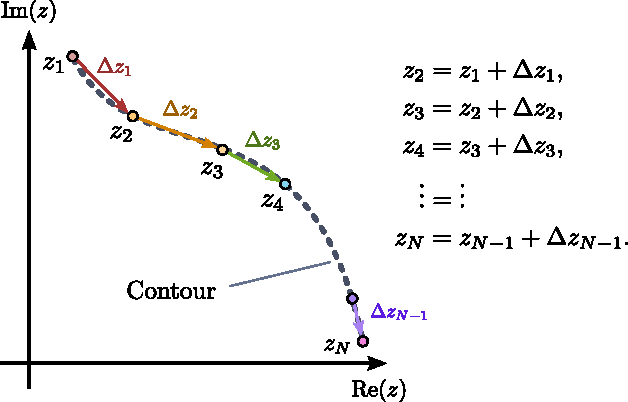
\includegraphics[width=0.7\textwidth]{complex_integral}
\end{figure}

\noindent
Then the sum we are interested in is
\begin{align}
  \sum_{n=1}^{N-1} \Delta z_n\; f(z_n) \;=\; \Delta z_1\, f(z_1) + \Delta z_2\, f(z_2) + \cdots + \Delta z_{N-1}\, f(z_{N-1}).
\end{align}
In the limit $N \rightarrow \infty$, each displacement $\Delta z_{n}$
becomes infinitesimal, and the sequence of points $\{z_1, z_2, \dots,
z_N\}$ becomes a continuous trajectory in the complex plane (see
Section 3.6). Such a trajectory is called a \textbf{contour}.

Let us denote a given contour by an abstract symbol, such as
$\Gamma$. Then the \textbf{contour integral} over $\Gamma$ is defined
as
\begin{align}
  \int_\Gamma \, f(z)\, dz \equiv \lim_{N \rightarrow \infty} \sum_{n=1}^{N-1} \Delta z_n\; f(z_n).
\end{align}
The symbol $\Gamma$ in the subscript of the integral sign indicates
that the integral takes place over the contour $\Gamma$. When defining
a contour integral, it is always necessary to specify which contour we
are integrating over.  Whereas for definite real integrals we only
needed to specify the end-points, for a contour integral it is not
enough to just state the end-points---we need to specify the entire
contour that starts and ends at those points!

Moreover, the specification of a contour must include the direction
along which the curve is traversed. If we integrate along the same
curve in the opposite direction, the value of the contour integral
switches sign (this is similar to swapping the end-points of a
definite real integral).

\begin{framed}\noindent
  \textit{Note}---Unlike a definite real integral, a contour integral
  does not have a geometrical interpretation in terms of an ``area
  under a curve''. It should be thought of as a generalization of the
  algebraic (as opposed to geometric) concept of an integral.
\end{framed}

\begin{framed}\noindent
  \textit{Note}---The contour should not be mistaken for the graph of
  the integrand! In many contour integration problems, the contour is
  sketched for you as a curve in the complex plane. Students who are
  new to contour integration sometimes mistake this for the graph of
  the integrand.
\end{framed}

\subsubsection{Contour integral along a parametric curve}
\label{contour-integral-along-a-parametric-curve}

Simple contour integrals can be calculated by \textbf{parameterizing
  the contour}.  Consider a contour integral
\begin{align*}
  \int_\Gamma \, dz \; f(z),
\end{align*}
where $f$ is a complex function of a complex variable and $\Gamma$ is
a given contour.

As discussed in Section 3.6, a trajectory in the complex plane can be
described by a complex function of a \textit{real} variable, $z(t)$:
\begin{align}
  \Gamma \equiv \Big\{z(t) \;\Big|\; t_1 < t < t_2\Big\}, \quad \mathrm{where}\;\; t \in \mathbb{R}, \,z(t) \in \mathbb{C}.
\end{align}
The real numbers $t_1$ and $t_2$ specify two complex numbers, $z(t_1)$
and $z(t_2)$, which are the end-points of the contour. The rest of the
contour consists of the values of $z(t)$ between those
end-points. Provided we can parameterize $\Gamma$ in such a manner,
the complex displacement $dz$ in the contour integral can be written
as
\begin{align}
  dz \rightarrow dt\, \frac{dz}{dt}.
\end{align}
Then we can express the contour integral over $\Gamma$ as a definite
integral over $t$:
\begin{align}
  \int_\Gamma dz\; f(z) = \int_{t_1}^{t_2} \; dt\; \frac{dz}{dt}\, f\big(z(t)\big).
\end{align}
This can then be calculated using standard integration techniques such
as those discussed in Chapter 3. A simple example is given in the next
section.

\subsubsection{A contour integral over a circular arc}
\label{arc-contour}

Let us use the method of parameterizing the contour to calculate the
contour integral
\begin{align}
  \int_{\Gamma[R, \theta_1,\theta_2]} dz\; z^n,\; n\in\mathbb{Z},
\end{align}
where the contour $\Gamma[R, \theta_1,\theta_2]$ is a
counter-clockwise arc of radius $R > 0$, from $z_1 = R e^{i\theta_1}$
to $z_2 = R e^{i\theta_2}$:

\begin{figure}[H]
  \centering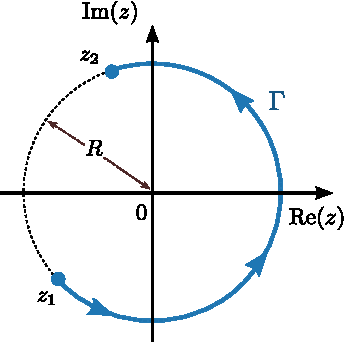
\includegraphics[width=0.34\textwidth]{complex_integral_example}
\end{figure}

\noindent
We can parameterize the contour as follows:
\begin{align}
  \Gamma[R, \theta_1,\theta_2] = \big\{z(\theta) \;\big|\; \theta_1 \le \theta \le \theta_2\big\}, \quad \mathrm{where}\;\, z(\theta) = R e^{i\theta}.
\end{align}
Then the contour integral can be converted into a definite integral
over the real variable $\theta$:
\begin{align}
  \int_{\Gamma[R, \theta_1,\theta_2]} dz\; z^n &= \int_{\theta_1}^{\theta_2}  d\theta \; z^n \; \frac{dz}{d\theta} \\
  &= \int_{\theta_1}^{\theta_2}  d\theta \; \left( Re^{i\theta}\right)^n\, \left(iR\, e^{i\theta}\right) \\
  &= i R^{n+1} \, \int_{\theta_1}^{\theta_2}  d\theta \; e^{i(n+1)\theta}.
\end{align}
To proceed, there are two cases that we must treat separately.  First,
for $n \ne -1$,
\begin{align}
  \int_{\theta_1}^{\theta_2} d\theta \; e^{i(n+1)\theta} = \left[\frac{e^{i(n+1)\theta}}{i(n+1)}\right]_{\theta_1}^{\theta_2} = \frac{e^{i(n+1)\theta_2} - e^{i(n+1)\theta_1}}{i(n+1)}.
\end{align}
Second, we have the case $n = -1$. This cannot be handled by the above
equations, since the factor of $n + 1$ in the denominator would
vanish.  Instead,
\begin{align}
  \int_{\theta_1}^{\theta_2} d\theta \; \left[e^{i(n+1)\theta} \right]_{n=-1} \; = \int_{\theta_1}^{\theta_2} d\theta \;=\; \theta_2 - \theta_1.
\end{align}
Putting the two cases together, we arrive at the result
\begin{align}
  \int_{\Gamma[\theta_1,\theta_2]} dz\; z^n = \left\{\begin{array}{ll}i(\theta_2 - \theta_1), & \mathrm{if}\;n = -1 \\ \displaystyle R^{n+1}\frac{e^{i(n+1)\theta_2} - e^{i(n+1)\theta_1}}{n+1},&\mathrm{if}\;n\ne -1.\end{array}\right.
\end{align}
The case where $\theta_2 = \theta_1 + 2\pi$ is of particular interest.
Here, $\Gamma$ forms a complete loop, and the result simplifies to
\begin{align}
  \oint_{\Gamma} dz\; z^n = \left\{\begin{array}{ll}2\pi i, & \mathrm{if}\;n = -1 \\ \displaystyle 0,&\mathrm{if}\;n\ne -1,\end{array}\right.
\end{align}
which is independent of $R$ as well as the choice of $\theta_1$ and
$\theta_2$.  (Here, the special integration symbol $\oint$ is used to
indicate that the contour integral is taken over a loop.)  This is a
very important result that we will make ample use of later.

By the way, what if $n$ is not an integer? In that case, the integrand
$z^n$ is multi-valued (as we saw in Chapter 8). This is problematic,
since the definition of a contour integral assumes the integrand is a
well-defined function. To get around this, we can specify a branch cut
and perform the contour integral with any of the branch functions of
$z^n$. So long as the branch cut avoids intersecting with the contour
$\Gamma$, the result obtained above by parametrizing the contour
integral remain valid.  However, $\Gamma$ cannot properly be taken
along a complete loop, as that would entail crossing the branch cut.

\subsection{Cauchy's integral theorem}
\label{cauchys-integral-theorem}

A \textbf{loop integral} is a contour integral taken over a loop in
the complex plane; i.e., with the same starting and ending point. We
have already seen the case of a circular loop integral in the previous
example.

Loop integrals play an important role in complex analysis. This
importance stems from the following property, known as
\textbf{Cauchy's integral theorem}:

\begin{framed}
If $f(z)$ is analytic everywhere inside a loop $\Gamma$, then $\displaystyle\oint_\Gamma dz\; f(z) = 0.$
\end{framed}

\subsubsection{Proof of Cauchy's integral theorem}
\label{proof-of-cauchys-integral-theorem}

Cauchy's integral theorem can be derived from
\href{http://en.wikipedia.org/wiki/Stokes'_theorem}{Stokes' theorem},
which states that for any differentiable vector field $\vec{A}(x,y,z)$
defined within a three-dimensional space, its line integral around a
loop $\Gamma$ is equal to the flux of its curl through any surface
enclosed by the loop.  Mathematically, this is stated as
\begin{align}
  \oint_\Gamma\, \vec{d\ell} \cdot \vec{A} = \int_{S(\Gamma)} d^2r \; \hat{n} \cdot \left(\nabla \times \vec{A}\right),
\end{align}
where $S(\Gamma)$ denotes a two-dimensional surface enclosed by the
loop $\Gamma$, and $\hat{n}$ denotes a normal vector sticking out of
the surface at each integration point.

We only need the 2D version of Stokes' theorem, in which both the loop
$\Gamma$ and the enclosed surface $S(\Gamma)$ are restricted to the
$x\mathrm{-}y$ plane, and $\vec{A}(x,y)$ likewise has no $z$
component.  Then Stokes' theorem simplifies to
\begin{align}
  \oint_\Gamma\, \vec{d\ell} \cdot \vec{A} = \int\!\!\!\int_{S(\Gamma)}\! dx \,dy \; \left(\frac{\partial A_y}{\partial x} - \frac{\partial A_x}{\partial y}\right).
\end{align}
Now consider a loop integral
\begin{align*}
  \oint_\Gamma dz \; f(z),
\end{align*}
where $\Gamma$ is a loop trajectory and $f(z)$ is some analytic
function that is analytic in the two-dimensional domain $S(\Gamma)$
enclosed by $\Gamma$. Let us decompose $f$ into its real and imaginary
parts,
\begin{align}
  f(x+iy) = u(x,y) + iv(x,y).
\end{align}
The analyticity of $f$ implies that the real functions $u$ and $v$ are
differentiable and obey the Cauchy-Riemann equations (see Section
6.3).

Let us manipulate the loop integral as follows:
\begin{align}
  \oint_\Gamma dz \, f(z) &= \oint_\Gamma \left(dx + i dy\right) \; \left(u + i v\right) \\
  &= \oint_\Gamma \Bigg(dx\, (u+iv) + dy\, (iu - v) \Bigg)  \\
  &= \oint_\Gamma \begin{bmatrix}dx\\dy\end{bmatrix} \cdot \begin{bmatrix}u + i v \\ iu - v\end{bmatrix}\\
      &= \oint_\Gamma \vec{d\ell} \cdot \vec{A}.
\end{align}

The last expression is a line integral involving the complex vector
field
\begin{align}
  \vec{A}(x,y) = \begin{bmatrix}u(x,y) + i v(x,y) \\ iu(x,y) - v(x,y)\end{bmatrix}.
\end{align}
Using Stokes' theorem in 2D, we convert this into the area integral
\begin{align}
  \int\!\!\!\int_{S(\Gamma)} dx \,dy \; \left(\frac{\partial A_y}{\partial x} - \frac{\partial A_x}{\partial y}\right) &= \int\!\!\!\int_{S(\Gamma)} dx \,dy \; \left[\left(i\frac{\partial u}{\partial x} - \frac{\partial v}{\partial x}\right) - \left(\frac{\partial u}{\partial y} + i \frac{\partial v}{\partial y}\right)\right] \\
  &= \int\!\!\!\int_{S(\Gamma)} dx \,dy \; \left[- \left(\frac{\partial v}{\partial x} + \frac{\partial u}{\partial y} \right) + i\left(\frac{\partial u}{\partial x} - \frac{\partial v}{\partial y}\right)\right].
\end{align}
On the last line, the two terms in parenthesis are both zero because,
according to the Cauchy-Riemann equations,
\begin{align}
  \frac{\partial u}{\partial x} = \frac{\partial v}{\partial y}\;\;\mathrm{and}\;\; \frac{\partial u}{\partial y} = -\frac{\partial v}{\partial x}.
\end{align}
Hence, the loop integral is zero. Q.E.D.

\subsubsection{Consequences of Cauchy's integral theorem}
\label{consequences-of-cauchys-integral-theorem}

Cauchy's integral theorem does not apply if the integrand $f(z)$ is
non-analytic somewhere inside the loop.  In particular, suppose $f(z)$
is not differentiable at one or more discrete points inside the loop, $\{z_1, z_2,
\dots\}$. Then we can show that
\begin{align}
  \oint_\Gamma dz\; f(z) \,=\, \sum_{n} \oint_{z_n} dz\; f(z),
  \label{eq:cit_result}
\end{align}
where $\oint_{z_n}$ denotes an integral over a loop of infinitesimal
radius around the $n$-th point of non-analyticity, in the \textit{same
  direction} (i.e., clockwise or counter-clockwise) as $\Gamma$.

The proof is based on the figure below. The red loop, $\Gamma$, is the
contour we want to integrate over. The integrand is analytic
throughout the enclosed area except at several discrete points, say
$\{z_1, z_2, z_3\}$. Let us define a new loop contour, $\Gamma'$,
shown by the blue loop. It follows the same curve as $\Gamma$ but with
the following differences: (i) it circles in the \textit{opposite}
direction from $\Gamma$, (ii) it contains tendrils that extend from
the outer curve to each point of non-analyticity, and (iii) each
tendril is attached to an infinitesimal loop encircling a point of
non-analyticity.

\begin{figure}[H]
  \centering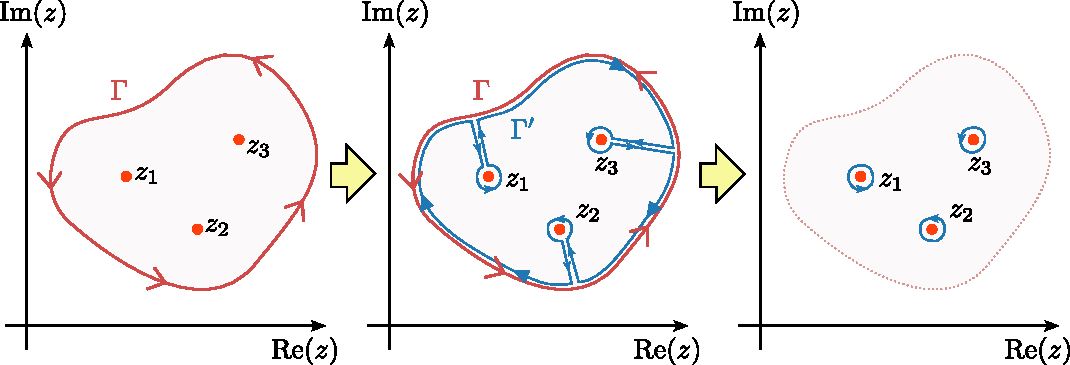
\includegraphics[width=0.95\textwidth]{contour_deformation}
\end{figure}

The loop $\Gamma'$ encloses no points of non-analyticity, so Cauchy's
integral theorem says that the integral over it is zero.  But the
contour integral over $\Gamma'$ can be broken up into three pieces:
(i) the part that follows $\Gamma$ but in the opposite direction, (ii)
the tendrils, and (iii) the infinitesimal inner loops:
\begin{align}
  \oint_{\Gamma'}& dz\; f(z)
\;\;= \;\; 0 \quad (\mathrm{by}\;\mathrm{Cauchy's}\;\mathrm{Integral}\;\mathrm{Theorem}) \\
&= \int_{\mathrm{big}\,\mathrm{loop}} dz\; f(z) + \int_{\mathrm{tendrils}} dz\; f(z) +\; \;\sum_{\mathrm{small~loop}~n}\;\; \oint_{z_n} dz\; f(z)
\end{align}
The first term is equal to the negative of $\oint_\Gamma dz \, f(z)$,
since it follows a contour that is just like $\Gamma$ except going the
other way.  The second term is zero, because each tendril consists of
two contours taken in opposite directions, which cancel.  Thus, the
above equation reduces to
\begin{align}
  \oint_\Gamma dz\; f(z) \,=\, \sum_n \oint_{z_n} dz\; f(z).
\end{align}
The loop contour integral over $\Gamma$ is equal to the sum of
infinitesimal loop contour integrals encircling each point of
non-analyticity. Notably, each of the infinitesimal loops circles in
the \textit{same} direction as $\Gamma$ (e.g., counter-clockwise in
the above figure).

Another way of thinking about this is that Cauchy's integral theorem
says regions of analyticity don't count towards the value of a loop
integral.  Hence, we can contract a loop across any domain in which
$f(z)$ is analytic, until the contour becomes as small as possible.
This contraction replaces $\Gamma$ with a discrete set of
infinitesimal loops enclosing the points of non-analyticity.

\subsection{Poles}
\label{poles}

In the previous section, we referred to situations where $f(z)$ is
non-analytic at discrete points.  ``Discrete'', in this context, means
that each point of non-analyticity is surrounded by a finite region
over which $f(z)$ is analytic, isolating it from other points of
non-analyticity. Such situations commonly arise from functions like
\begin{align}
  f(z) = \frac{1}{(z-z_0)^n}, \quad \mathrm{where}\;\; n\in\{1,2,3,\dots\}.
\end{align}
For $z = z_0$, this function is non-analytic because its value is
singular.  We say that there is a \textbf{pole} at $z_0$.  The integer
$n$ is called the \textbf{order} of the pole.

\subsubsection{Residue of a simple pole}
\label{residue-of-a-simple-pole}

Poles of order 1 are called \textbf{simple poles}, and they are of
special interest. If a function has a simple pole at $z_0$, it can be
approximated near the pole as
\begin{align}
  f(z) \approx \frac{A}{z-z_0}.
\end{align}
The complex numerator $A$ is called the \textbf{residue} of the pole
(so-called because it's what's left-over if we take away the singular
factor corresponding to the pole.) We denote the residue of a function
$f(z)$ at $z = z_0$ by
\begin{align}
  \mathrm{Res}\big[\,f(z), \, z = z_0\,\big].
\end{align}
Note that if $f$ is analytic at $z_0$ (i.e., there is no pole there),
then $\mathrm{Res}[f(z), z = z_0] = 0$.

\begin{framed}\noindent
  \textit{Example}---Consider the function
  \begin{align}
    f(z) = \frac{5}{i-3z}.
  \end{align}
To find the pole and residue, divide the numerator and denominator by $-3$:
\begin{align}
  f(z) = \frac{-5/3}{z-i/3}.
\end{align}
Thus, there is a simple pole at $z = i/3$ and
\begin{align}
  \mathrm{Res}\big[\,f(z),\, z = i/3\,\big] = - 5/3.
\end{align}
\end{framed}

\begin{framed}\noindent
  \textit{Example}---Consider the function
  \begin{align}
    f(z) = \frac{z}{z^2 + 1}.
  \end{align}
To find the poles and residues, we factorize the denominator:
\begin{align}
  f(z) = \frac{z}{(z+i)(z-i)}.
\end{align}
Hence, there are two simple poles, at $z = \pm i$.

To find the residue at $z = i$, separate the divergent part from the
rest of the expression:
\begin{align}
  f(z) &= \frac{\left(\frac{z}{z+i}\right)}{z-i} \\
  \Rightarrow\quad \mathrm{Res}\big[\,f(z), z=i\,\big]
  &= \left[\frac{z}{z+i}\right]_{z=i} = 1/2.
\end{align}
Likewise, for the other pole at $z = -i$,
\begin{align}
  \mathrm{Res}\big[\,f(z), \, z = -i\,\big] = \left[\frac{z}{z-i}\right]_{z=-i} = 1/2.
\end{align}
\end{framed}

\subsubsection{The residue theorem}
\label{the-residue-theorem}

In Section~\ref{arc-contour}, we used contour parameterization to
calculate
\begin{align}
  \oint_{\Gamma} \frac{dz}{z} = 2\pi i,
\end{align}
where $\Gamma$ is a counter-clockwise circular loop centered on the
origin. This holds for any (non-zero) loop radius.  Combining this
result with Eq.~\eqref{eq:cit_result}, we obtain the \textbf{residue
  theorem}:

\begin{framed}
  \noindent
  For any analytic function $f(z)$ with a simple pole at $z_0$,
  \begin{align}
    \oint_{\Gamma[z_0]} dz \; f(z) = \pm 2\pi i \, \mathrm{Res}\big[\,f(z)\,, z = z_0 \,\big],
  \end{align}
  where $\Gamma[z_0]$ denotes an infinitesimal loop around $z_0$.  The
  $+$ sign holds for a counter-clockwise loop, and the $-$ sign for a
  clockwise loop.
\end{framed}

\noindent
Hence, we arrive at an integration technique called the
\textbf{calculus of residues}:

\begin{enumerate}
\item Identify the poles of $f(z)$ in the domain enclosed by $\Gamma$.

\item Check that these are all simple poles, and that $f(z)$ has no other non-analytic behaviors (e.g. branch cuts) in the enclosed region.

\item At each pole $z_n$, calculate the residue $\mathrm{Res}[f(z),\, z = z_n]$.

\item The value of the loop integral is
  \begin{align}
    \oint_\Gamma dz\; f(z) = \pm 2\pi i \sum_n \mathrm{Res}\big[\,f(z),\,z = z_n\,\big].
  \end{align}
  The plus sign holds if $\Gamma$ is counter-clockwise, and the minus
  sign if it is clockwise.
\end{enumerate}

\subsubsection{Example of the calculus of residues}
\label{residues-example}

Consider
\begin{align}
  f(z) = \frac{1}{z^2 + 1} = \frac{1}{(z + i)\,(z-i)}.
\end{align}
By inspection, we can identify two poles: one at $+i$, with residue
$1/2i$, and the other at $-i$, with residue $-1/2i$. The function is
analytic everywhere else.

Suppose we integrate $f(z)$ around a counter-clockwise contour
$\Gamma_1$ that encloses only the pole at $+i$, as indicated by the
blue curve in the figure below:

\begin{figure}[ht]
  \centering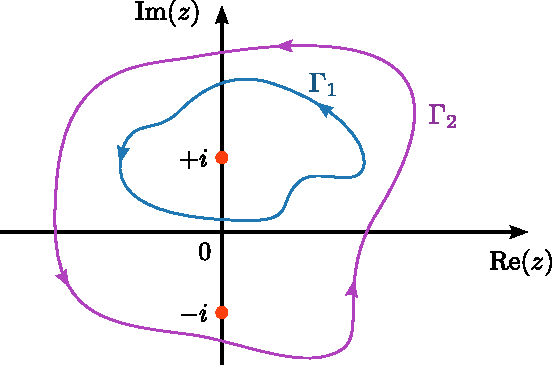
\includegraphics[width=0.45\textwidth]{contour_example1}
\end{figure}

\clearpage
According to the residue theorem,
\begin{align}
  \oint_{\Gamma_1}dz \; f(z) &= 2\pi i\, \mathrm{Res}\big[\,f(z),\,z = i\,\big] \\
  &= 2\pi i \cdot \frac{1}{2i} \\
  & = \pi.
\end{align}
On the other hand, suppose we integrate around a contour $\Gamma_2$
that encloses \textit{both} poles, as shown by the purple curve. Then
the result is
\begin{align}
  \oint_{\Gamma_2}dz \; f(z) = 2\pi i \cdot \left[\frac{1}{2i} - \frac{1}{2i}\right] = 0.
\end{align}

\subsection{Using contour integration to solve definite integrals}
\label{using-contours-to-solve-integrals}

One of the principal applicaitons of the calculus of residues is to
help us handle definite integrals \textit{over the real domain} by
converting them into contour integrals, which are then solved with the
residue theorem.

As an example, consider the definite integral
\begin{align}
  \int_{-\infty}^\infty \frac{dx}{x^2 + 1}.
\end{align}
This integral is taken over real values of $x$, and we previously
solved it using a change of variables in Section 2.4.  Now let's see
how to solve it using contour integration.

First, generalize the integrand from a function of $x$ to an analytic
function of $z$.  (This procedure is called \textbf{analytic
  continuation}.)  Usually, we choose the new (complex) integrand so
that it reduces to the old integrand for real values of $z$. In this
case, let
\begin{align}
  \frac{1}{x^2 + 1} \rightarrow \frac{1}{z^2 + 1}.
\end{align}
This is just the integrand we dealt with in the previous section.

We now have to choose the contour.  The usual procedure is to define a
loop contour such that one segment of the loop is the real line (from
$-\infty$ to $+\infty$), and the other segment ``doubles back'' in the
complex plane to close the loop.  This is called \textbf{closing the
  contour}.

Here, we choose to close the contour along an anticlockwise
semicircular arc in the upper half of the complex plane, as shown
below:

\begin{figure}[ht]
  \centering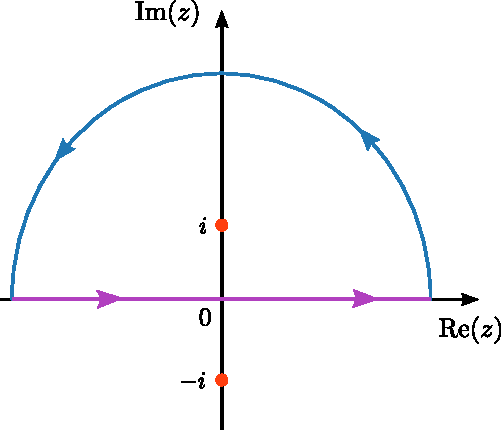
\includegraphics[width=0.45\textwidth]{closing_contour}
\end{figure}

\noindent
This loop integral can be decomposed into a sum of two contour integrals:
\begin{align}
  \oint \frac{dz}{z^2 + 1} = \int_{-\infty}^\infty \frac{dx}{x^2 + 1} \;+\; \int_{\mathrm{arc}} \frac{dz}{z^2 + 1}.
\end{align}
The first term is equal to the integral we're interested in. The
second term is a contour integral along the big arc, and we can show
that it goes to zero.  To see why, observe that along an arc of radius
$R$, the magnitude of the integrand goes as $1/R^{2}$, while the $dz$
gives another factor of $R$ (see the earlier example of parameterizing
a contour integral over an arc in Section~\ref{arc-contour}), so the
overall integral goes as $1/R$, which vanishes as $R \rightarrow
\infty$.

Now to evaluate the loop contour integral. Since the loop encloses the
pole at $z = +i$,
\begin{align}
  \oint \frac{dz}{z^2+1} = 2\pi i \; \mathrm{Res}\left[\,\frac{1}{z^2 + 1}, \, z = i\,\right] = \pi.
\end{align}
The loop is counterclockwise, so we take the positive sign for the
residue theorem. Hence,
\begin{align}
  \int_{-\infty}^\infty \frac{dx}{x^2 + 1} = \pi.
\end{align}
As an exercise, you can verify that closing the contour in the lower
half-plane gives the same result.

\vskip 0.3in

\subsubsection{Jordan's lemma}
\label{jordans-lemma}

Before proceeding to more complicated uses of contour integration, we
must introduce an important result called \textbf{Jordan's lemma}:

\begin{framed}
\noindent
Let
\begin{align}
  I = \int_C dz \; e^{iqz} \,g(z),
\end{align}
where $q$ is any positive real constant, and the contour $C$ which is a semi-circular arc of radius $R$ in the upper half-plane, centered at the origin. Then
\begin{align}
  \text{If}\;\; \big|\,g(z)\,\big| < g_{\mathrm{max}} \;\;\;\text{for all}\;\;z \in C \;\;\;\Rightarrow \;\;\; I \rightarrow 0 \;\;\mathrm{as}\;\; g_{\mathrm{max}} \rightarrow 0.
\end{align}
\end{framed}

\noindent
In other words, if the factor of $g(z)$ in the integrand does not blow
up along the arc contour (i.e., its value is bounded), then in the
limit where the bounding value goes to zero, the value of the entire
integral vanishes.

Usually, the limit of interest is when the radius of the arc goes to
infinity. Even if the integrand vanishes in that limit, it may not be
obvious that the integral $I$ vanishes, as the integration is taken
along an arc of infinite length (so we have a $0\times\infty$ sort of
situation). Jordan's lemma then proves useful, because it provides a
rigorous criterion for us to conclude that $I$ should vanish.

The proof for Jordan's lemma is tedious, and we will not go into its
details.

 
For integrands containing a prefactor of $e^{-iqz}$ rather than
$e^{iqz}$ (again, where $q \in \mathbb{R}^+$), a different version of
Jordan's lemma holds, referring to an arc contour $C'$ in the
\textit{lower} half-plane:

\begin{framed}
\noindent
Let
\begin{align}
  I = \int_C dz \; e^{-iqz} \,g(z),
\end{align}
where $q$ is any positive real constant, and the contour $C$ which is a semi-circular arc of radius $R$ in the lower half-plane, centered at the origin. Then
\begin{align}
  \text{If}\;\; \big|\,g(z)\,\big| < g_{\mathrm{max}} \;\;\;\text{for all}\;\;z \in C \;\;\;\Rightarrow \;\;\; I \rightarrow 0 \;\;\mathrm{as}\;\; g_{\mathrm{max}} \rightarrow 0.
\end{align}
\end{framed}

\noindent
This is easily seen by doing the change of variable $z \rightarrow -z$
on the original form of Jordan's lemma.

As a convenient way to remember which variant of Jordan's lemma to
use, think about which end of imaginary axis causes the exponential
factor to vanish:
\begin{align}
  e^{iqz}\big|_{z = i\infty}\;\; = e^{-\infty} = 0\quad &\Rightarrow \;\; e^{iqz} \;\;\;\,\text{vanishes far above the origin}. \\
  e^{-iqz}\big|_{z = -i\infty} = e^{-\infty} = 0\quad &\Rightarrow \;\; e^{-iqz} \;\;\textrm{vanishes far below the origin}.
\end{align}
Hence, for $e^{iqz}$ (where $q$ is any positive real number), the
suppression occurs in the upper-half-plane. For $e^{-iqz}$, the
suppression occurs in the lower-half-plane.

\subsubsection{A contour integral using Jordan's lemma}
\label{a-contour-integral-using-jordans-lemma}

Consider the integral
\begin{align}
  I = \int_{-\infty}^\infty dx\; \frac{\cos(x)}{4x^2 + 1}.
\end{align}
One possible approach is to break the cosine up into $(e^{ix} +
e^{-ix})/2$, and do the contour integral on each piece separately.
Another approach, which saves a bit of effort, is to write
\begin{align}
  I = \mathrm{Re} \left[ \int_{-\infty}^\infty dx\; \frac{e^{ix}}{4x^2 + 1}\right].
\end{align}
To do the integral, close the contour in the upper half-plane:

\begin{figure}[ht]
  \centering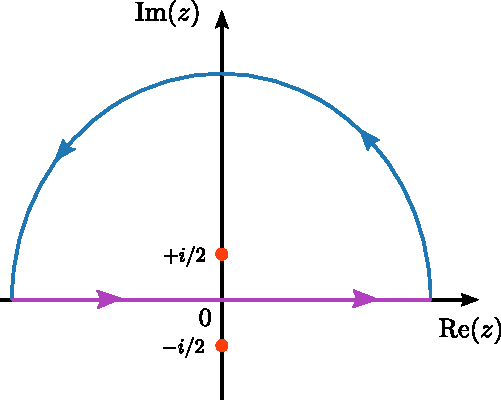
\includegraphics[width=0.47\textwidth]{contour_example3}
\end{figure}

\noindent
Then
\begin{align}
  \oint dz \; \frac{e^{iz}}{4z^2 + 1} = \int_{-\infty}^\infty dx\; \frac{e^{ix}}{4x^2 + 1} + \int_{\mathrm{arc}} dz \; \frac{e^{iz}}{4z^2 + 1}.
\end{align}
On the right-hand side, the first term is what we want. The second
term is a counter-clockwise arc in the upper half-plane. According to
Jordan's lemma, this term goes to zero as the arc radius goes to
infinity, since the rest of the integrand goes to zero for large
$|z|$:
\begin{align}
  \left|\frac{1}{4z^2 + 1}\right| \sim \frac{1}{4|z|^2} \rightarrow 0 \quad \mathrm{as} \;|z| \rightarrow \infty.
\end{align}
As for the loop contour, it can be evaluated using the residue
theorem:
\begin{align}
  \oint dz \; \frac{e^{iz}}{4z^2 + 1} &= 2\pi i \; \mathrm{Res}\left[\frac{1}{4}\, \frac{e^{iz}}{(z+i/2)(z-i/2)}\,,\; z = \frac{i}{2} \;\right] \\
  &= 2\pi i \; \frac{e^{-1/2}}{4i}.
\end{align}
Hence,
\begin{align}
  I = \mathrm{Re}\left[\frac{\pi}{2\sqrt{e}}\right]= \frac{\pi}{2\sqrt{e}}.
\end{align}
In solving the integral this way, we must close the contour in the
upper half-plane because our choice of complex integrand was bounded
in the upper half-plane.  Alternatively, we could have chosen to write
\begin{align}
  I = \mathrm{Re} \left[ \int_{-\infty}^\infty dx\; \frac{e^{-ix}}{4x^2 + 1}\right],
\end{align}
i.e., with $e^{-ix}$ rather than $e^{ix}$ in the numerator.  In that
case, Jordan's lemma tells us to close the contour in the lower
half-plane.  The arc in the lower half-plane vanishes, as before,
while the loop contour is clockwise (contributing an extra minus sign)
and encloses the lower pole:
\begin{align}
  \oint dz \frac{e^{-iz}}{4z^2 + 1} &= -2\pi i \, \mathrm{Res}\left[ \frac{e^{-iz}}{4z^2 + 1}\,, \; z = -\frac{i}{2} \right] \\
  &= - 2\pi i \frac{e^{-1/2}}{-4i} \\
  &= \frac{\pi}{2\sqrt{e}}.
\end{align}
Taking the real part, we obtain the same result as before.

\subsection{Principal value integrals (optional topic)}
\label{principal-value-integrals}

Sometimes, we come across integrals that have poles lying on the
desired integration contour.

As an example, consider
\begin{align}
  I = \int_{-\infty}^\infty dx\; \frac{\sin(x)}{x}.
\end{align}
Because of the series expansion of the sine function (see Section
1.2), the integrand does not diverge at $x = 0$, and the integral is
in fact convergent. The integral can be solved without using complex
numbers by using the arcane trick of differentiating under the
integral sign (see Section 2.6).  But it can also be solved via
contour integration.

We start by writing
\begin{align}
  I = \mathrm{Im}[I'], \quad \mathrm{where}\;\;\; I' = \int_{-\infty}^\infty dx\; \frac{e^{ix}}{x}.
\end{align}
We want to calculate $I'$ with the help of contour integration.  But
there's something strange about $I'$: the complex integrand has a pole
at $z = 0$, right on the real line!

To handle this, we split $I'$ into two integrals, one going over
$-\infty < x < -\epsilon$ (where $\epsilon$ is some positive
infinitesimal), and the other over $\epsilon < x < \infty$:
\begin{align}
  I' &= \lim_{\epsilon \rightarrow 0} \left[ \int_{-\infty}^{-\epsilon} dx\; \frac{e^{ix}}{x} + \int_{\epsilon}^\infty dx\; \frac{e^{ix}}{x}\right] \\
  &\equiv \mathcal{P} \int_{-\infty}^\infty dx\; \frac{e^{ix}}{x}.
\end{align}
In the last line, the notation $\mathcal{P}[\cdots]$ is short-hand for
this procedure of ``chopping away'' an infinitesimal segment
surrounding the pole.  This is called \textbf{taking the principal
  value} of the integral.  (Note: even though this bears the same name
as the previously-discussed ``principal values'' for multi-valued
complex operations from Chapter 8, the two concepts are unrelated.)

Now consider the loop contour shown in the figure below.  The loop
follows the principal-value contour along the real axis, skips over
the pole at $z = 0$ and arcs back along the upper half-plane.  Since
it encloses no poles, the loop integral vanishes by Cauchy's integral
theorem.

\begin{figure}[ht]
  \centering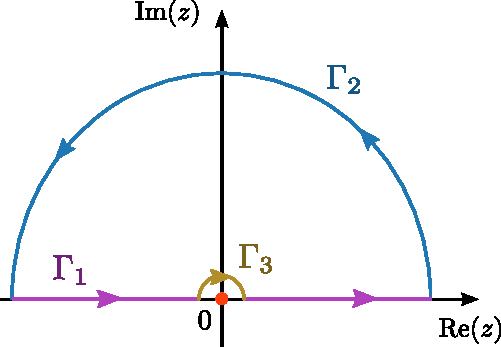
\includegraphics[width=0.47\textwidth]{principal_value_integral}
\end{figure}

\noindent
This loop can be decomposed into several sub-contours:
\begin{enumerate}
\item  $\Gamma_1$, consisting of the segments along the real axis.
\item $\Gamma_2$, the large counter-clockwise semi-circular arc.
\item $\Gamma_3$, the infinitesimal clockwise semi-circular arc that skips around $z = 0$.
\end{enumerate}

\noindent
The integral over $\Gamma_1$ is the principal-value integral we are
interested in.  The integral over $\Gamma_2$ vanishes by Jordan's
lemma. The integral over $\Gamma_3$ can be calculated by
parameterization:
\begin{align}
  \int_{\Gamma_3} \frac{e^{iz}}{z} &= \lim_{\epsilon \rightarrow 0} \int_{\pi}^{0} \frac{e^{i\epsilon \exp(i\theta)}}{\epsilon e^{i\theta}} \left(i\epsilon e^{i\theta}\right) d\theta \\
  &= i \int_{\pi}^0 d\theta \\
  &= - i\pi.
\end{align}
Intutively, since encircling a pole anticlockwise gives a factor of
$2\pi i$ times the residue (which is 1 in this case), a clockwise
semi-circle is associated with a factor of $- i \pi$. Finally, putting
everything together,
\begin{align}
  \underbrace{\int_{\Gamma_1 + \Gamma_2 + \Gamma_3} f(z) dz}_{ =~0~(\text{Cauchy's integral theorem})} = \underbrace{\int_{\Gamma_1} f(z) dz}_{=~I'} + \underbrace{\int_{\Gamma_2} f(z) dz}_{=~0~(\text{Jordan's lemma})} + \underbrace{\int_{\Gamma_3} f(z) dz.}_{=~-i \pi}
\end{align}
Hence,
\begin{align}
  I = \mathrm{Im}(I') = \mathrm{Im}(i\pi) = \pi.
\end{align}
This agrees with the result obtained by the method of differentiating
under the integral sign from Section 2.6.

Alternatively, we could have chosen the loop contour so that it skips
\textit{below} the pole at $z = 0$.  In that case, the loop integral
would be non-zero, and can be evaluated using the residue theorem.
The final result is the same.

\subsection{Exercises}
\label{exercises}

\begin{enumerate}
\item
  Is the concept of a contour integral well-defined if the integrand
  $f(z)$ is non-differentiable along the contour? Why or why not?

\item
  In Section~\ref{using-contours-to-solve-integrals}, we dealt with
  the integral
  \begin{equation}
    \int_{-\infty}^\infty \frac{dx}{x^2 + 1}.
  \end{equation}
  Redo this calculation, but this time close the contour in the lower
  half-plane.  Show that the result is the same.
  \hfill{\scriptsize [solution~available]}

\item
  Calculate
  \begin{equation}
    \int_{-\infty}^\infty dx\; \frac{1}{x^4 + 1}.
  \end{equation}

\item
  Calculate
  \begin{equation}
    \int_{-\infty}^\infty dx\; \left[\frac{\sin(x)}{x}\right]^2.
  \end{equation}

\item
  Calculate
  \begin{equation}
    \int_0^\infty dx \frac{x^{\lambda}}{x+1}, \;\;\mathrm{where}\; -1 < \lambda < 0.
  \end{equation}
  Hint: place the integrand's branch cut along the positive real axis.

\item
  Solve the definite integral
  \begin{equation}
    I = \int_0^{2\pi} \frac{d\phi}{\cos\phi+3},
  \end{equation}
  via the following steps. First, show that along a unit circle in the
  complex plane centered at the origin,
  \begin{equation}
    \cos\phi = \frac{1}{2}\left(z+\frac{1}{z}\right),
  \end{equation}
  where $z(\phi) = \exp(i\phi)$. Then define a complex function $f(z)$
  such that the loop integral $\oint f(z) \;dz,$ taken over the
  circular contour, is equal to $I$. Hence, calculate
  $I$.
  \vskip -0.05in
  \hfill{\scriptsize [solution~available]}
  
\item
    Suppose \(f(z)\) is analytic everywhere in the upper half-plane,
  including the real line, and that its magnitude vanishes as \(1/|z|\)
  or faster as \(|z| \rightarrow \infty\). Find the value of the
  principal-value integral
  \begin{equation}
    \mathcal{P}\left[\int_{-\infty}^\infty \frac{f(x)}{x-a} dx \right],
  \end{equation}
  where \(a\) is some real constant. Hence, prove that the real and
  imaginary parts of \(f\) along the real line are related by
  \begin{align}
    \mathrm{Re}\big[f(x)\big]
    &= \;\;\,\frac{1}{\pi} \mathcal{P}\left[\int_{-\infty}^\infty
      \frac{\mathrm{Im}[f(w)]}{w-x} dw\right]
    \\ \mathrm{Im}\big[f(x)\big]
    &= -\frac{1}{\pi} \mathcal{P}\left[\int_{-\infty}^\infty
      \frac{\mathrm{Re}[f(w)]}{w-x} dw\right].
  \end{align}
  These are called the \textbf{Kramers-Kronig relations}. In physics,
  these relations impose important constraints on the frequency
  dependence of the real and imaginary parts of the dielectric
  function (the square of the complex refractive index).
  \vskip -0.05in
  \hfill{\scriptsize [solution~available]}
\end{enumerate}


\end{document}
